\uuid{CnBv}
\titre{Etude d'un fonction de deux variables}
\chapitre{Fonction de plusieurs variables}
\niveau{L2}
\module{Analyse}
\sousChapitre{Dérivées partielles}
\theme{}
\auteur{Grégoire MENET}
\datecreate{2025-04-16}
\organisation{AMSCC}

\difficulte{}
\contenu{
	
	\texte{
		On considère trois fonctions de deux variables \(f\), \(g\) et \(h\) dont les expressions ne sont pas connues.
		Les domaines de définition de ces fonctions sont respectivement :
		\[
		D_f = \left\{(x,y) \in \mathbb{R}^2 \ \middle|\ x + y \geq 0 \text{ et } x^2 \neq y \right\}
		\]
		\[
		D_g = \left\{(x,y) \in \mathbb{R}^2 \ \middle|\ x \neq y \text{ et } x^2 + y^2 > 1 \right\}
		\]
		\[
		D_h = \left\{(x,y) \in \mathbb{R}^2 \ \middle|\ x + y \neq 1 \right\}
		\]
	}
	
	\begin{enumerate}
		\item \question{Tracer ces domaines de définition. Pour chacun de ces domaines, déterminer s'il est ouvert, fermé ou ni l'un ni l'autre. Justifier brièvement.}
		\indication{Tracer les ensembles en considérant les inégalités et exclusions indiquées dans chaque domaine. Analyser les conditions d'inclusion des frontières pour déterminer si les ensembles sont ouverts ou fermés.}
		\reponse{
				

					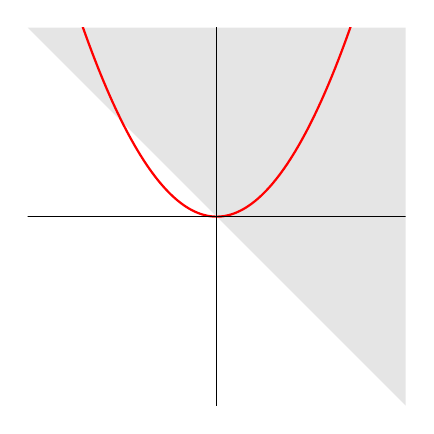
\begin{tikzpicture}[scale=1.2]
						\fill[gray!20] (-2,-2) -- (2,-2) -- (2,2) -- (-2,2) -- cycle;
						\fill[white] (-2,-2) -- (2,-2) -- (2,2) -- (-2,2) -- cycle;
						\clip (-2,-2) rectangle (2,2);
						
						\fill[gray!20, domain=-2:2, variable=\x]
						plot ({\x}, {-1*\x}) -- (2,2) -- (-2,2) -- cycle;
						
						% exclusion y = x^2
						\draw[red, thick, domain=-1.5:1.5, samples=100] plot (\x, {\x*\x});
						
						\draw[->] (-2.2,0) -- (2.2,0) node[below right] {$x$};
						\draw[->] (0,-2.2) -- (0,2.2) node[left] {$y$};
						\node at (0,-2.5) {$D_f$};
						%\node at (1.5,1.8) {\Large $D_f$}
					\end{tikzpicture}
					%\caption*{\textbf{Domaine $D_f$} : $x+y \geq 0$ sans la courbe $y = x^2$}


					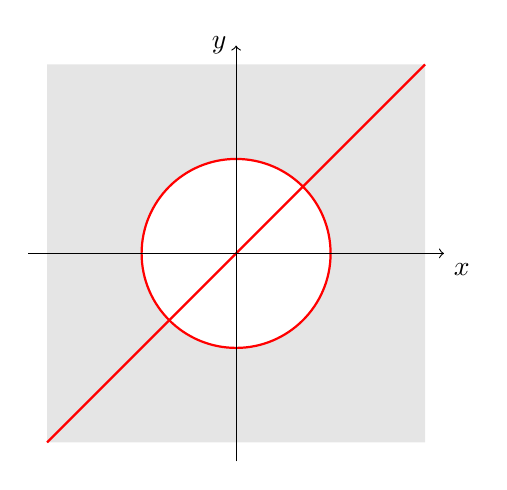
\begin{tikzpicture}[scale=1.2]
						\fill[gray!20, even odd rule] 
						(0,0) circle (1.0)
						(-2,-2) rectangle (2,2);
						\draw[red, thick] (0,0) circle (1);   
						\draw[red, thick, domain=-2:2] plot (\x, {\x}); % x = y
						
						\draw[->] (-2.2,0) -- (2.2,0) node[below right] {$x$};
						\draw[->] (0,-2.2) -- (0,2.2) node[left] {$y$};
						%\node at (0,-2.5) {$D_g$};
					\end{tikzpicture}
					%\caption*{\textbf{Domaine $D_g$} : extérieur du disque unité sans la droite $x = y$}


					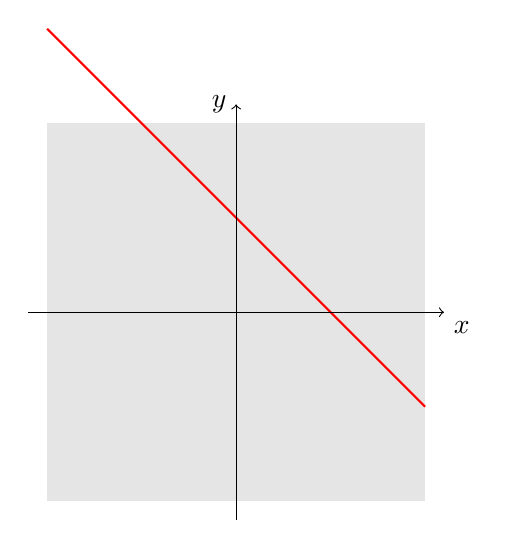
\begin{tikzpicture}[scale=1.2]
						\fill[gray!20] (-2,-2) rectangle (2,2);
						\draw[red, thick, domain=-2:2] plot (\x, {1 - \x}); % x + y = 1
						
						\draw[->] (-2.2,0) -- (2.2,0) node[below right] {$x$};
						\draw[->] (0,-2.2) -- (0,2.2) node[left] {$y$};
						%\node at (0,-2.5) {$D_h$};
					\end{tikzpicture}
					%\caption*{\textbf{Domaine $D_h$} : tout $\mathbb{R}^2$ sauf la droite $x + y = 1$}

			Les courbes en rouge sont exclues du domaine de définition.\\
			Le domaine de $f$ contient seulement une partie de son bord, il est donc ni ouvert ni fermé. Les domaines de $g$ et de $h$ ne contiennent pas leurs bords, ils sont donc ouverts.}
		
		\item \question{On sait que \(f\) est de classe \(\mathcal{C}^1\) sur son domaine de définition et que \(f(x^2,0)=\frac{1}{x^3}\) pour \(x>0\). À l'aide de la dérivée d'une composée, déduire \(\frac{\partial f}{\partial x}(1,0)\).}
		\indication{Appliquer la règle de dérivation en chaîne à l'expression \(f(x^2,0)\) et égaler la dérivée obtenue à celle de \(\frac{1}{x^3}\) pour \(x>0\).}
		\reponse{On pose $F(x) = f(x^2, 0)$, avec $F(x) = \frac{1}{x^3}$ pour $x > 0$.\\
			
			D'après la formule de la dérivée composée :
			\[
			F'(x) = \frac{\partial f}{\partial x}(x^2, 0) \cdot 2x
			\]
			
			On évalue en $x = 1$ :
			\[
			-\frac{3}{1^4} = \frac{\partial f}{\partial x}(1, 0) \cdot 2 \Rightarrow \frac{\partial f}{\partial x}(1, 0) = -\frac{3}{2}
			\]
			
			\[
			\boxed{\frac{\partial f}{\partial x}(1, 0) = -\frac{3}{2}}
			\]}
		
		\item \question{On sait que \(\lim\limits_{(x,y)\rightarrow(2,0)} g(x,y)=\ln\left(\frac{2}{3}\right)\) et que les dérivées partielles de \(g\) en \((2,0)\) existent. Peut-on en conclure que \(g(2,0)=\ln\left(\frac{2}{3}\right)\) ? Justifier votre réponse.}

		\reponse{Non, une fonction qui admet des dérivées partielles en un point n'est pas nécessairement continue en ce point. On n'a donc pas nécessairement $\lim_{(x,y)\rightarrow(2,0)} g(x,y)=g(2,0)$.}
		
		\item \question{À laquelle des trois fonctions correspond le graphe suivant ? Justifier.
	
		\includegraphics[width=250pt]{exam}	
	}
		
		\reponse{Le graphe correspond à la fonction $h$. En effet on voit que la fonction correspondant au graphe n'est pas définie sur la droite d'équation $x + y = 1$, ce qui coïncide avec le domaine de définition de $h$.}
		

	\end{enumerate}
	
}
